\chapter{Kết luận}
\label{chap:ket-luan}

\section{Kết luận và đóng góp}
\label{sec:ket-luan}\label{sec:dong-gop}\label{chap:dong-gop}

Tiểu luận đặt câu hỏi ``grounded hay guessed?'' cho SemLoc~\cite{yang2026semloc} và so nó với cách làm đơn giản của nhiều
lập trình viên: chạy kiểm thử, đưa kết quả thất bại cho LLM. Nhóm tính lại từ nhật ký, chạy lại mã của tác giả, kiểm
tra lại nhãn, lặp ba lần có kiểm định và tách đóng góp của từng tín hiệu. Câu trả lời cho bốn câu hỏi nghiên cứu như sau;
Hình~\ref{fig:cai-tien} tóm tắt mức hơn của FailLoc so với SemLoc trên mọi bộ nhãn và trên lỗi thật.
\begin{itemize}
\item \textbf{RQ1}: tính lại từ nhật ký khớp, chạy lại thì không; điểm thưởng không được mô tả quyết định dòng đầu; kiểm
chứng phản thực tế không đổi thứ hạng; mã chấm điểm lạc quan với gỡ lỗi chia đôi, bi quan với SBFL; gần một nửa nhãn bị
dời khi rà soát (Mục~\ref{sec:overclaim}).
\item \textbf{RQ2}: FailLoc thắng SemLoc ở Acc@1 trên cả ba bộ nhãn và rẻ hơn nhiều.
\item \textbf{RQ3}: kiểm thử thất bại là tín hiệu chính, độ phủ không giúp; CovGate chỉ tăng Acc@3 của SemLoc, còn
FailLoc+Verify, FailLoc+Vote và phân tích tĩnh không cải thiện được; không cách nào thu hẹp khoảng cách với FailLoc.
\item \textbf{RQ4}: trên lỗi thật kết quả cùng chiều nhưng chưa đủ mẫu; đổi tên làm yếu phổ ràng buộc nhưng không ảnh
hưởng dòng đoán hay FailLoc+Cov; ở cả năm mô hình, bỏ điểm thưởng đều làm Acc@1 của SemLoc giảm.
\end{itemize}

\begin{figure}[H]
\centering
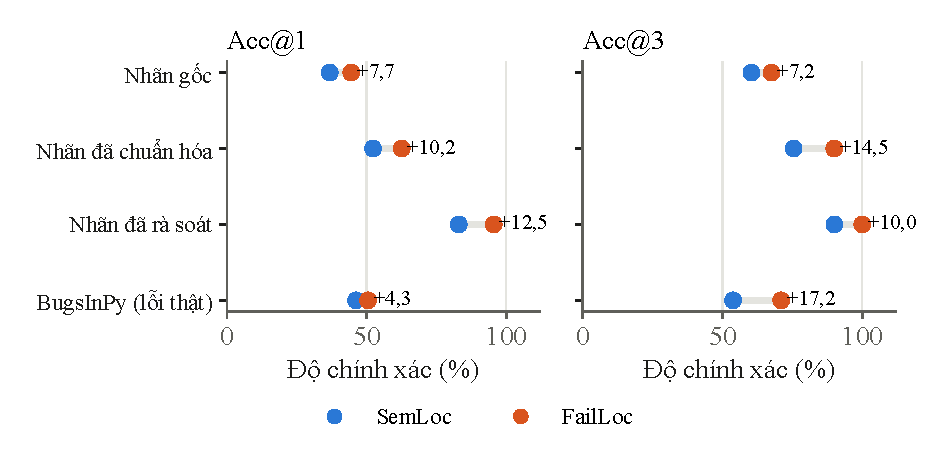
\includegraphics{../generated/vi/fig_improvement.pdf}
\caption{FailLoc so với SemLoc trên cùng chương trình và cùng mô hình: ba bộ nhãn (tập test) và lỗi thật BugsInPy}
\label{fig:cai-tien}
\end{figure}

Mỗi đóng góp có bằng chứng là tệp dữ liệu trong kho mã (\texttt{data/}) và điều kiện bác bỏ đi kèm.
\begin{itemize}
\item \textbf{C1 (RQ1). Kiểm tra lại SemLoc.} Một điểm thưởng không được mô tả trong bài báo đặt dòng tự đoán lên hạng
  1; Acc@1 của SemLoc (\RqTwoRepairedAllSemlocAccOneMean\%) là của dòng đoán, SemLoc−Bonus đạt
  \RqTwoRepairedAllSemlocNoPriorAccOneMean\%, và bước vá thử chiếm \CostCfSharePct\% lượt gọi LLM mà không đổi thứ hạng nào.
  Điểm thưởng là lựa chọn thiết kế; tuyên bố quá mức (overclaim) là gọi thứ hạng đó là neo vào bằng chứng thực thi.
  Ngoài ra \LabaudAllMoved{}/\LabaudAllN{} nhãn bị dời khi rà soát; nhóm công bố hai bộ nhãn: đã chuẩn hóa (\GtConfirmedN{}
  xác nhận, \GtCorrectedN{} dời, chỉ kiểm thử quyết định) và đã rà soát (vòng duyệt mù:
  \BlindBlindAllMatchReviewed{}/\BlindBlindAllNReviewed{} câu trả lời trùng nhãn).
\item \textbf{C2 (RQ2). Phương pháp FailLoc}: một prompt có kiểm thử thất bại hơn SemLoc ở Acc@1 trên cả ba bộ nhãn
  (\RqTwoRepairedAllLlmTestsDAccOne{} [\RqTwoRepairedAllLlmTestsDAccOneLo; \RqTwoRepairedAllLlmTestsDAccOneHi] điểm trên
  bộ đã chuẩn hóa) với \CostLlmTestsTokensK{} so với \CostSemlocTokensK{} nghìn token mỗi chương trình.
\item \textbf{C3 (RQ3). Vì sao FailLoc thắng}: kiểm thử thất bại là tín hiệu chính (Acc@3
  \AblRepairedAllTestsEffectDAccThree{} so với LLM-Direct); FailLoc+Cov, FailLoc+Vote, FailLoc+Verify, ruff và pyrefly
  không giúp, CovGate chỉ thêm \RqTwoRepairedAllCovgateDAccThree{} điểm Acc@3 cho SemLoc. Cơ chế: kiểm thử ``sửa được''
  \PavmechReviewedOtherLineFixable\% lần thử tại dòng không có lỗi (tập dev, nhãn đã rà soát; Mục~\ref{chap:that-bai}).
\item \textbf{C4 (RQ4). Kiểm chứng độ bền}: FailLoc vẫn thắng SemLoc trên lỗi thật BugsInPy (Acc@3
  \BipAllLlmTestsAccThreeMean\% so với \BipAllSemlocPriorAccThreeMean\%), gần như không đổi khi mã bị đổi tên định danh
  (Acc@3 \RenRepairedLlmTestsDAccThree{} điểm), và không thua SemLoc ở cả năm họ mô hình.
\end{itemize}

Kèm theo các đóng góp là bảng kiểm tra bảy mục (phá hòa, mẫu số, dòng lỗi kiểm chứng, loại bỏ thành phần ẩn, lặp và
kiểm định, chi phí, so với một prompt có kiểm thử thất bại) và gói tái hiện (Docker chạy không cần mạng, bộ đệm lượt gọi
LLM để phát lại, tệp duyệt nhãn và macro sinh tự động cho mọi con số). Nhóm đề xuất mọi đánh giá định vị lỗi bằng LLM áp
dụng bảng kiểm tra này. Nội dung chính của báo cáo được
viết lại thành bài báo tiếng Anh (mã nguồn \LaTeX{} ở \texttt{docs/report/paper-en} trong kho mã) để nộp arXiv, cùng gói tái hiện.

\section{Triết lý khoa học}
\label{sec:triet-ly}

Ở mọi chỗ cần phán xử, nhóm để kiểm thử quyết định và để LLM chỉ sinh ứng viên; khi kiểm thử không đủ (lỗi hai dòng, lỗi
thiếu mã, bản sửa bù trừ), nhóm dùng người duyệt và nói rõ phần nào do ai quyết định. Nếu một phương pháp tuyên bố neo lập
luận vào thực thi thì phần neo đó phải được đo: phân rã đóng góp và loại bỏ từng thành phần biến câu hỏi ``phương pháp có
tốt không'' thành ``phần nào làm nó tốt''. Tái hiện gồm cả việc hiểu vì sao ra con số công bố, ngoài việc khớp được nó. Một quy
trình nhiều bước chỉ đáng giá khi thắng cách đơn giản người làm nghề vẫn dùng. Mỗi khẳng định đi kèm điều kiện bác bỏ và
khoảng tin cậy, đơn vị lấy mẫu là chương trình, kết quả âm tính cũng được báo cáo. Bộ dữ liệu cũng là một giả thuyết: nhãn
có thể sai, và cả bộ phán định lẫn vòng rà soát của nhóm đều có giới hạn.

\section{Hạn chế và hướng phát triển}
\label{sec:moi-de-doa}\label{sec:huong-phat-trien}

Các kết luận đến từ một mô hình chính, chương trình một hàm có kiểm thử rõ ý định, và 31 lỗi thật của một dự án. Cụ thể,
bốn nhóm hạn chế sau có thể ảnh hưởng tới tính hợp lệ của kết quả.

\begin{itemize}
\item \textbf{Nhãn}: bộ phán định chấp nhận bản sửa bù trừ và có thể thiên về phương pháp dùng độ phủ; Acc@1 chặt phụ thuộc
  quy ước đầu khối/thân khối; nhãn đã rà soát do LLM đề xuất nên có nguy cơ vòng tròn (duyệt mù chỉ trên
  \BlindBlindAllPrograms{} chương trình, \BlindAnswersExcluded{} câu bị loại). Mọi kết quả chính vì vậy được báo cáo cả
  trên bộ gốc và bộ đã chuẩn hóa.
\item \textbf{Prompt và tên kiểm thử}: prompt của FailLoc do nhóm viết, không tinh chỉnh; tên kiểm thử của SemFault-250
  ``nói hộ'' ý định, nhóm chưa chạy thí nghiệm giấu tên kiểm thử.
\item \textbf{Lỗi thật}: chỉ 31 lỗi của một dự án (youtube-dl), hàm đích lấy từ bản sửa nên định vị cấp hàm chưa được đánh giá.
\item \textbf{Mô hình}: một mô hình chính; nghiên cứu năm mô hình chạy trên một tập con, chưa có khoảng tin cậy, và
  FailLoc trên GPT-6 luna gọi qua OpenAI API thay vì Codex.
\end{itemize}

Các hướng phát triển đi ra từ chính những hạn chế này: (i) định vị lỗi cấp dự án: thu hẹp từ kho mã xuống một hàm trước khi hỏi LLM; (ii) thí nghiệm giấu tên kiểm thử để đo phần
thông tin tên kiểm thử ``nói hộ''; (iii) bộ kiểm thử chặt hơn (sinh kiểm thử phân biệt các bản sửa) để kiểm chứng vị trí lỗi
bằng thực thi có ý nghĩa; (iv) thêm nhiều bộ dữ liệu, gồm lỗi thật từ nhiều dự án và ngôn ngữ khác ngoài Python, để chạy các phương pháp trên quy mô
lớn hơn, với FailLoc làm mốc.
